\documentclass{beamer}
\usepackage{HECbeamer}
\usepackage{icomma}
% \usepackage{pgfpages}
% \pgfpagesuselayout{4 on 1}[letterpaper, landscape, border shrink=5mm]
\title[\color{white}{MATH 60604 \S~4c - Exemple de régression logistique}]{\texorpdfstring{MATH 60604 \\Modélisation statistique \\ \S~4c - Exemple de régression logistique}{MATH 60604 \\Modélisation statistique \\ \S~4c - Exemple de régression logistique}}
\author{}
\institute{HEC Montréal\\
Département de sciences de la décision}
\date{} 

\begin{document}
\frame{\titlepage}

\begin{frame}[fragile]
\frametitle{Achat suite au visionnement d'une publicité}

Dans le cadre d'une étude, des sujets ont navigué sur un site web
qui contenait, entre autres, une publicité pour des bonbons. Pendant la
navigation, un dispositif de suivi occulaire enregistrait l'endroit où se posait le regard du
sujet. On a ainsi pu mesurer le temps de fixation du sujet. Un logiciel d'analyse des expressions faciales (FaceReader) a aussi servi à mesurer l'émotion du sujet pendant le visionnement de la publicité.
 
\vp


Supposons qu'au lieu de mesurer l'intention d'achat par questionnaire au moment où nos participants était au laboratoire, \alert{nous les avions plutôt contacté un mois plus tard pour voir s'ils avaient acheté le produit depuis leur visite}.
\end{frame}
\begin{frame}
\frametitle{Nombre d'achats}
Le jeu de données \texttt{intention} contient deux autres variables:

\bi\item \code{achat}: variable binaire, \texttt{1} si le sujet à acheté des bonbons, \texttt{0} sinon.
\item \texttt{nachat}: nombres d'achats de l'item
\ei
\begin{center}
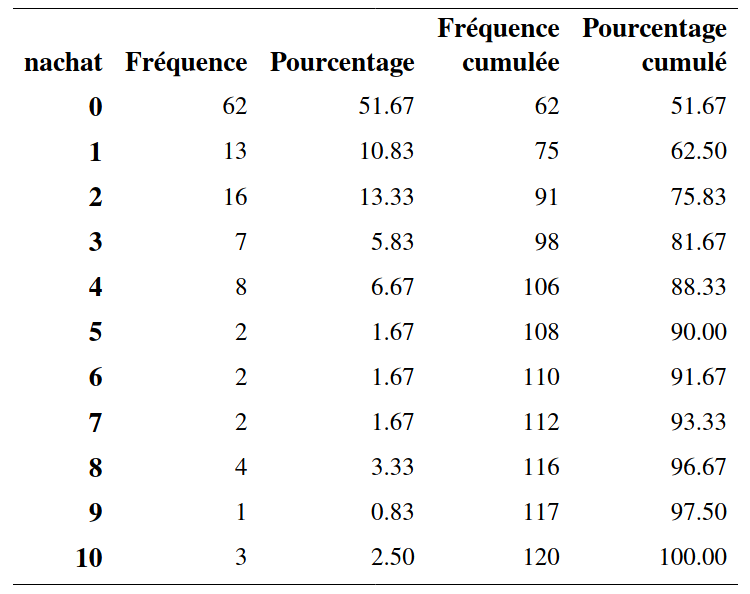
\includegraphics[width = 0.6\linewidth]{img/c4/diapos8-e2}
\end{center}
{\small 
La variable \texttt{nachat} varie de $0$ à $10$ avec une moyenne de $1,71$ achat par participant(e). $51,7$\% des sujets n'ont fait aucun achat.
}
\end{frame}
% 
% \begin{frame}[fragile]
% \frametitle{Modèle pour données de dénombrement}
% \bi
% % \item We revisit the example of fixation time on a candy advertisement. 
% % \item Suppose that this time we've measured the \alert{number of times a person bought the product in the month following the study}. 
% \item The response variable of interest $Y$ is therefore a \alert{count} variable, \code{nitem}.
% \item The predictor variables are the same , namely \texttt{sex}, \texttt{age}, \texttt{revenue}, \texttt{educ}, \texttt{marital}, \texttt{fixation}, and \texttt{emotion}. 
% % \item It might be possible to model a transformation of the response variable, e.g., $\log(Y+1)$, as a function of the predictor variables -- however, we cannot compare them because of the transformation. 
% % \item  We will compare results from ordinary linear regression to those obtained here. 
% % \item However, with this kind of discrete variable, the distribution of the outcome is often skewed to the right, meaning that other kinds of generalized linear models may be more suitable.
% \ei
% 
% \end{frame}
% 

\begin{frame}[fragile]
\frametitle{Nombre d'achats suite au visionnement d'une publicité}
On se concentre sur \texttt{acaht} comme variable réponse. Les variables explicatives sont les même que précédemment, à savoir
 {\small 
\bi
\item {\code{fixation}}: durée totale de fixation de la publicité (en secondes).
\item {\code{emotion}}: une mesure de la valence durant la fixation, soit le ratio
de la probabilité d’une émotion positive sur la probabilité d’une émotion négative
\item {\code{sexe}}: sexe du sujet, soit homme (\code{0}) ou femme (\code{1}).
\item {\code{age}}: âge (en années).
\item {\code{revenu}}: variable catégorique indiquant le revenu annuel du sujet; un parmi
{ \footnotesize
\be
\item $[0,  20\ 000]$;
\item $[20\ 000,  60\ 000]$;
\item $60\ 000$ et plus.
\ee
}
\item {\code{educ}}: variable catégorique indiquant le niveau d'éducation, soit le plus haut grade obtenu
{ \footnotesize \be
\item secondaire ou moindre;
\item collégial;
\item universitaire.
\ee}
\ei
}
\end{frame}
\begin{frame}[fragile]
\frametitle{Modèle logistique pour les achats}
On dénote $\pi=\P{Y=1\mid \mathbf{X}}$ la probabilité d'acheter le produit dans le mois suivant l'étude conditionnelles aux variables explicatives, selon le modèle

\begin{align*}
\logit(\pi)&=\beta_0 + \beta_1 \code{sexe} + \beta_2 \code{age} + \beta_3 \code{revenu}_1 + \beta_4 \code{revenu}_2 \\
&\qquad + \beta_5 \code{educ}_1 + \beta_6 \code{educ}_2 + \beta_7 \code{statut} \\
&\qquad + \beta_8 \code{fixation} + \beta_9 \code{emotion}.
\end{align*}



\end{frame}

\begin{frame}[fragile]
\frametitle{Code \SASlang pour la régression logistique}
\bi
\item Les paramètres $\bs{\beta}$ ne sont vraiment interprétables qu'à l'échelle exponentielle.
\item La procédure \code{logistic} avec les options \code{plcl plrl expb} permet d'obtenir les estimés $\exp(\hat{\beta})$ et des intervalles de confiance basés sur la vraisemblance pour ces paramètres.
\item Avec \code{proc logistic}, la paramétrisation habituelle pour les variables catégorielles est obtenue avec l'option \texttt{param=glm}.
\ei
\begin{tcolorbox}[colback=white, colframe=hecblue, title=Code \SASlang{} pour \code{proc logistic}]
\begin{verbatim}
proc logistic data=modstat.intention;
class educ revenu / param=glm;
model achat(ref="0")=sexe age revenu educ statut
    fixation emotion / plcl plrl expb;
run;
\end{verbatim}
\end{tcolorbox}
\end{frame}

\begin{frame}
\frametitle{Sortie \SASlang{} de la procédure \texttt{logistic}}
\begin{center}
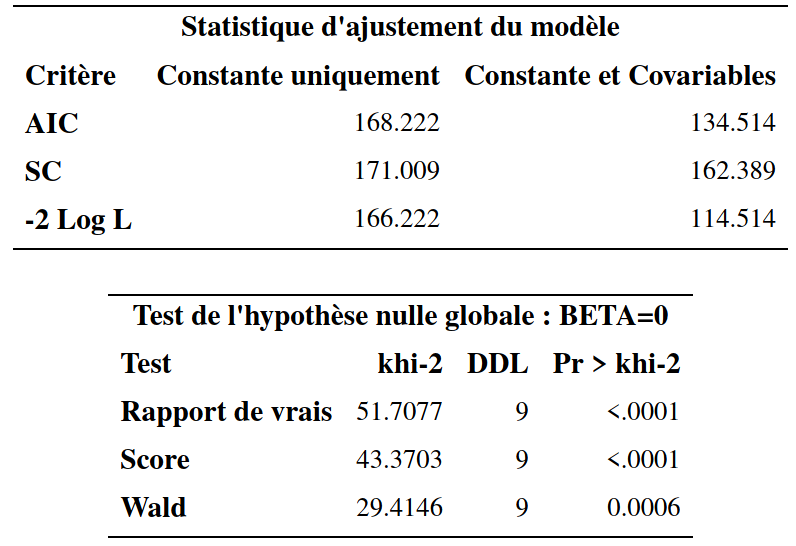
\includegraphics[width=0.50\textwidth]{img/c4/diapos8-e11}
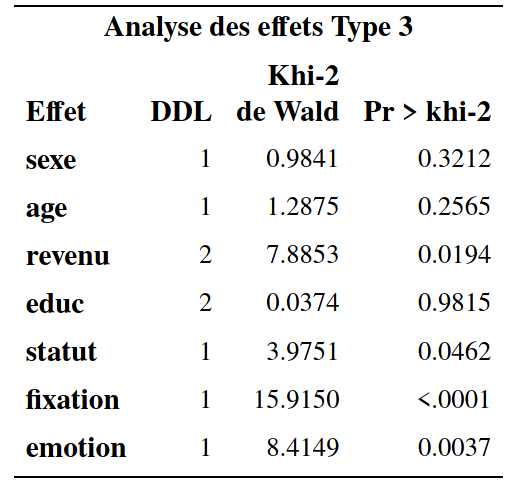
\includegraphics[width=0.35\textwidth]{img/c4/diapos8-e12}
\end{center}
{\small 
\bi \item Des diagnostics sur la qualité de l'ajustement sont rapportés pour le modèle sans covariables qui inclut uniquement l'ordonnée à l'origine (probabilité constante de succcès) et le modèle ajusté.
\item En plus des critères d'information, la sortie contient les statistiques de tests (Wald, score, rapport de vraisemblance) pour l'hypothèse nulle, $\Hy_0: \beta_1 = \cdots = \beta_p = 0$.
\item Le tableau de significativité des paramètres (effets type III) est basé sur des statistiques de Wald (pour des tests de rapport de vraisemblance, utiliser la procédure \texttt{genmod} avec l'option \texttt{type3}).
\ei
}
\end{frame}
\begin{frame}
\frametitle{Estimés des paramètres}
\begin{center}
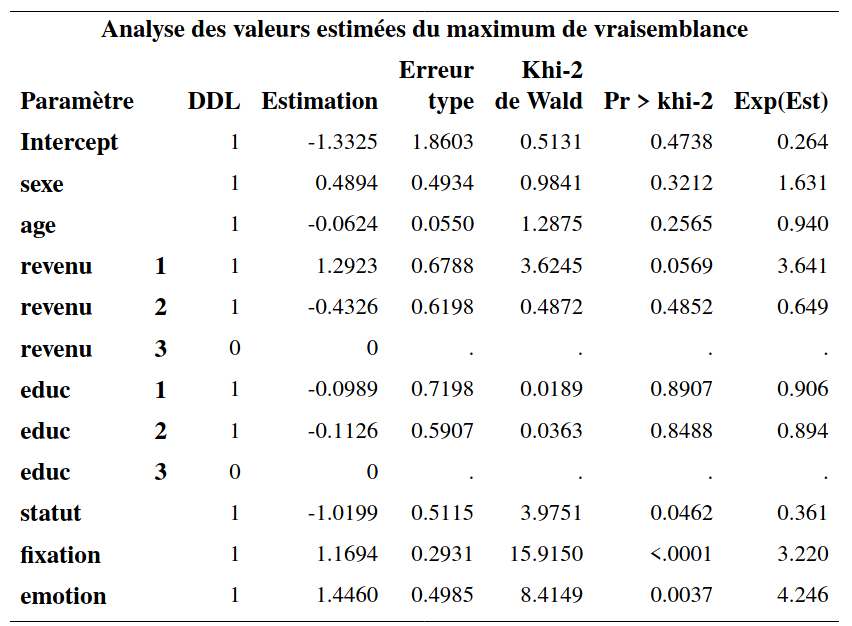
\includegraphics[width = 0.85\textwidth]{img/c4/diapos8-e13}
\end{center}
{\footnotesize 
\bi
\item La dernière colonne du tableau contient $\exp(\hat{\beta}_j)$ (option \code{expb}).
\item Les tests de significativité pour $\beta_i=0$ sont basés sur des statistiques de Wald.
\ei

}
\end{frame}

\begin{frame}
 \frametitle{Tableau des estimés des coefficients}
 \begin{center}
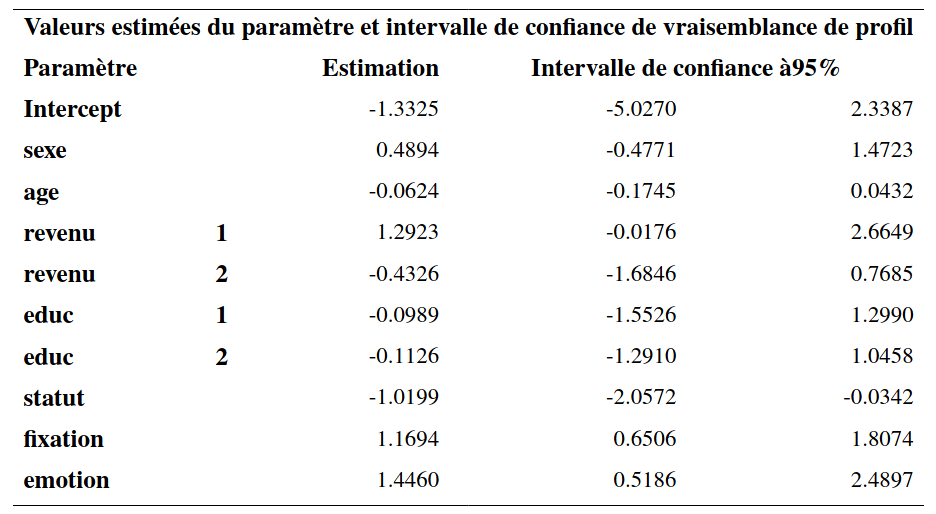
\includegraphics[width = 0.8\linewidth]{img/c4/diapos8-e14.png}
\end{center}

\end{frame}
\begin{frame}{Tableau des estimés des coefficients à l'échelle exponentielle}
\begin{center}
 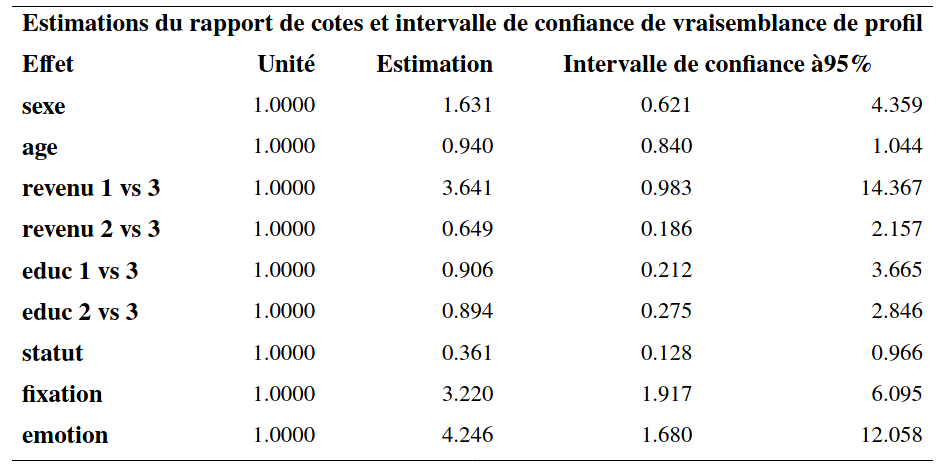
\includegraphics[width = 0.8\linewidth]{img/c4/diapos8-e15.png}
\end{center}
{\footnotesize 
\bi\item À l'échelle exponentielle, les paramètres ne sont pas significatifs à niveau 5\% si $1$ est inclut dans l'intervalle de confiance.
\item 
Pour obtenir les intervalles de confiance basés sur les rapports de vraisemblance, spécifier l'option \texttt{plrl}.
\ei
}
\end{frame}

\begin{frame}[fragile]
\frametitle{Interprétation des paramètres}
\bi
\item $\exp(\hat{\beta}_{\code{sex}})=1.631$: la cote d'achat pour les femmes (\code{sexe=1}) est $1.631$ fois plus élevée que pour les hommes, toute autre chose étant égale par ailleurs. La probabilité que les femmes achètent au moins un item est plus élevée que celle des hommes après ajustement. 
\item $\exp(\hat{\beta}_{\code{age}})=0.94$: pour deux personnes qui ne différent que d'un an, la cote pour l'achat de la personne plus âgée est $0.94$ celle de la personne plus jeune, une diminution de $6\%$, \textit{ceteris paribus}.

\item Toutes choses étant égales par ailleurs, la cote pour l'achat augmente de $\exp(\hat{\beta}_{\code{fixation}})=3.22$ pour toute augmentation du temps de fixation de une seconde.

\ei
\end{frame}
\begin{frame}[fragile]
\frametitle{Comparaison des niveaux de \code{revenu}}
\bi
\item Le coefficient pour $\code{revenu}_1$  est relatif au niveau \code{revenu=3} et $\exp(\hat{\beta}_{\code{revenu}_1})=3,641$: la cote d'achat pour les sujets à faible revenu (\code{revenue=1}) est $3,641$ fois plus élevée que celle des personnes à revenu élevé (\code{revenu=3}), \textbf{toutes choses étant égales par ailleurs}. 
\item Pour obtenir le rapport de cotes entre les niveaux $1$ et $2$ de \code{revenu}, on pourrait réajuster le modèle en changeant la catégorie de référence.
\item On peut également calculer le rapport de rapports de cotes de $3,641/0,649=5,61$; on a donc que la cote de succès pour le niveau de revenu $1$ est $461\%$ plus élevée que celle pour la classe de revenu moyen $2$, toute autre chose étant égale par ailleurs.
\ei
\end{frame}


\begin{frame}[fragile]
\frametitle{Représentation visuelle des rapports de cote}
\begin{center}
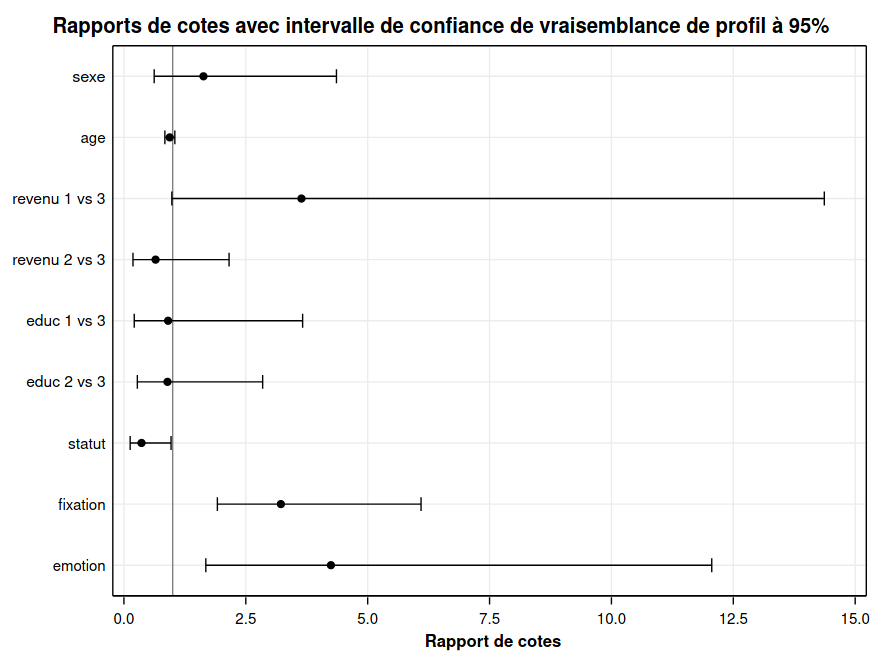
\includegraphics[width = 0.8\linewidth]{img/c4/diapos8-e16}

\end{center}
{\footnotesize 

Les intervalles de confiance calculés à partir de la vraisemblance profilée sont \textbf{invariants aux reparamétrisations}: on obtient un intervalle de confiance pour $\exp(\beta_k)$ en appliquant la fonction exponentielle à chaque borne de l'intervalle pour $\beta_k$.

}
\end{frame}


% 
% 
% \begin{frame}
% \frametitle{Interprétation de la sortie \texttt{lsmeans}}
% \begin{center}
% 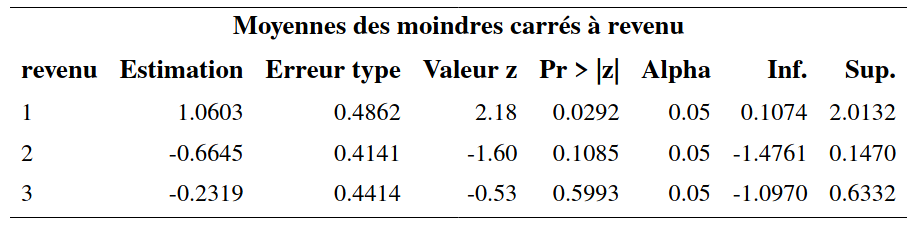
\includegraphics[width = 0.8\linewidth]{img/c4/diapos8-e17}
% \end{center}
% La colonne ``\textbf{Estimation}'' donne l'estimé  \textbf{non-conditionnel} de la \alert{probabilité moyenne} transformée, $\logit(\pi)$, pour chaque niveau de revenu.
%  {\small 
% \bi
% \item Pour \code{revenu=1}, la probabilité moyenne d'achat est
% \begin{align*}
% \expit(0,59)=\frac{\exp({0,59})}{1+\exp({0,59})}=0,64.
% \end{align*}
% \item Pour \code{revenu=2}, la probabilité moyenne d'achat est $\expit(-0,9188)=0,28$.
% \item Pour \code{revenu=3}, la probabilité moyenne d'achat est  $\expit(-0,5082)=0,37$.
% \ei
% 
% Cette sortie est similaire à celle d'une ANOVA à un facteur (\texttt{revenu}) sur l'échelle transformée.
% }
% \end{frame}
% 
% 
% \begin{frame}
% \frametitle{Différences des paires pour les niveaux de revenu}
% \begin{center}
% 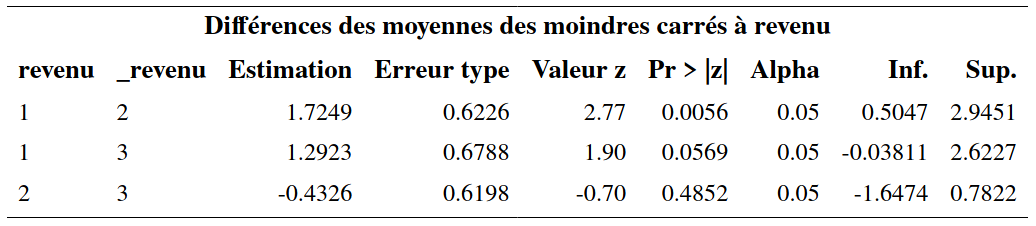
\includegraphics[width = 0.8\linewidth]{img/c4/diapos8-e18}
% 
% \end{center}
% \bi
% \item La colonne ``\textbf{Estimation}'' dans le tableau montre la différence (à l'échelle logit) des probabilités \textbf{non-conditionnelles} entre chaque catégorie de revenu.
% \item Les intervalles de confiance sont basés sur des statistiques de Wald, on ne rejette pas l'hypothèse d'absence de différence à niveau 5\% si zéro est dans l'intervalle de confiance.
% \item Les gens qui ont un faible niveau de revenu une probabilité d'achater beaucoup plus élevée que ceux de la classe de revenu moyen.
% \ei
% \end{frame}
% 
% 


\begin{frame}[fragile]
\frametitle{Prédiction}
\bi
\item La régression logistique est fréquemment utilisée en apprentissage machine pour la classification.
\bi
 
\item si on veut prédire la valeur de $Y$ (zéro ou un) pour de nouvelles observations pour lesquelles on a observé les covariables.
\ei
\item On peut aisément \textbf{prédire} à partir du modèle de régression logistique ajusté, sachant que
\begin{align*}
\pi_i=\P{Y_i=1\mid \mathbf{X}_i}=\frac{\exp(\beta_0+ \beta_1 \mathrm{X}_{i1}+\cdots + \beta_p \mathrm{X}_{ip})}{1+\exp(\beta_0+ \beta_1 \mathrm{X}_{i1}+\cdots + \beta_p \mathrm{X}_{ip})}.
\end{align*}
\item Si on substitue $\hat{\bs{\beta}}$ en lieu et place des paramètres inconnus, on obtient un estimé de la probabilité de succès,  $\hat{\pi}_i=\widehat{\p}(Y_i=1\mid \mathbf{X}_i)$.
\item On peut utiliser cet estimé $\widehat{\pi}_i$ pour prédire la valeur de $Y_i$ avec un point de coupure $c$, 
\bi
 \item si $\hat{\pi}_i > c$, on prédit $\hat{Y}_i=1$.
\item si $\hat{\pi}_i \leq c$, on prédit $\hat{Y}_i=0$.
\ei
\ei
\end{frame}

\begin{frame}[fragile]
 \frametitle{Séparation (quasi)-complète de variables}
 \bi \item Dans certaines applications, il existe des combinations de variables explicatives qui permettent de prédire exactement certaines ou toutes les valeurs de $Y \in \{0, 1\}$.
 \bi \item Par exemple, un sondage à la sortie des urnes dans lequel chaque vote correspond à l'affiliation politique rapportée.
 \ei
  \item  Bien que les prédictions soient toujours valides, la séparation (quasi)-complète est problématique pour l'interprétation (une bonne analogie est l'impact de la collinéarité).
\item L'estimaté du maximum de vraisemblance est infini pour certains paramètres (cas limite) ou encore n'est pas unique --- cela empêche le calcul d'erreurs-type, etc. 
\ei
\end{frame}
\begin{frame}[fragile]
\frametitle{Détection et remèdes pour la séparation (quasi)-complète}
 \bi \item Il est facile de diagnostiquer les problèmes dans les logiciels.
 \item Par exemple, \Rlang{} imprime le message 
 {\footnotesize  
\begin{verbatim}
 Warning message: glm.fit: des probabilités ont été ajustées 
 numériquement à 0 ou 1
\end{verbatim}
} dans la console, tandis que dans  \SASlang{}, on obtient
{\footnotesize 
 \begin{verbatim}
 Complete separation of data points detected. 
 WARNING: The maximum likelihood estimate does not exist.
 \end{verbatim}
 }
\item On peut restaurer l'identifiabilité des paramètres en pénalisation la fonction de log-vraisemblance. La correction de Firth est une solution populaire qui permet d'obtenir des coefficients finis et uniques. 
 \bi \item option \texttt{firth} dans la procédure \SASlang{} \texttt{logistic} 
 \item la fonction \texttt{logistf} du paquetage éponyme dans \Rlang{}
 \ei
 \ei
\end{frame}

\end{document}
